\let\negmedspace\undefined
\let\negthickspace\undefined
\documentclass[journal,12pt,onecolumn,article]{IEEEtran}
\usepackage{cite}
\usepackage{color,soul}
\usepackage{amsmath,amssymb,amsfonts,amsthm}
\usepackage{algorithmic}
\usepackage{graphicx}
\usepackage{textcomp}
\usepackage{xcolor}
\usepackage{subcaption}
\usepackage{txfonts}
\usepackage{listings}
\usepackage{enumitem}
\usepackage{mathtools}
\usepackage{gensymb}
\usepackage{comment}
\usepackage[breaklinks=true]{hyperref}
\usepackage{tkz-euclide} 
\usepackage{listings}
\usepackage{multicol}
\usepackage{gvv}       
\usepackage[dvipsnames]{xcolor}
\def\inputGnumericTable{}                                
\usepackage[latin1]{inputenc}                            
\usepackage{color}                                       
\usepackage{array}                                       
\usepackage{longtable}                                   
\usepackage{calc}                                        
\usepackage{multirow}                                    
\usepackage{hhline}                                      
\usepackage{ifthen}                                      
\usepackage{lscape}
\usepackage{float}
\newtheorem{theorem}{Theorem}[section]
\newtheorem{problem}{Problem}
\newtheorem{proposition}{Proposition}[section]
\newtheorem{lemma}{Lemma}[section]
\newtheorem{corollary}[theorem]{Corollary}
\newtheorem{example}{Example}[section]
\newtheorem{definition}[problem]{Definition}
\newcommand{\BEQA}{\begin{eqnarray}}
\newcommand{\EEQA}{\end{eqnarray}}
\newcommand{\define}{\stackrel{\triangle}{=}}
\theoremstyle{remark}
\newtheorem{rem}{Remark}
\begin{document}
\bibliographystyle{IEEEtran}
\vspace{3cm}
\title{Gate-ASSIGNMENT-1}
\author{EE24BTECH11043 - Murra Rajesh Kumar Reddy}
\maketitle
\bigskip
\begin{enumerate}
	\item In a machine shop, pins of $15$ mm diameter are produced at a rate of 1000 per month and the consumed at a rate of 500 per month. The production and the consumption continue simultaneously till the maximum inventory is reached. Then inventory is allowed to reduced to zero due to consumption. The lot size of production is 1000. If backlog is not allowed, the maximum inventory level is 
	\begin{enumerate}
		\item $400$
		\item $500$
		\item $600$
		\item $700$
	\end{enumerate}
\item The net requirements of an item over 5 consecutive weeks are 50-0-15-20-20. The invetory carrying cost and odering cast are RE. 1 per item per week and RS. 100 per order respectively. Starting inventory is zero. Use "Least Unit Cost Technique" for developing the plan. The cost of plan (in Rs.) is 
	\begin{enumerate}
		\item $200$
		\item $250$
		\item $255$
		\item $260$
	\end{enumerate}
		\section*{Common data questions}
		Common Data questions for $71,72,73$ \\
		A gear set has a pinion with 20 teeth and a gear with 40 teeth. The pinion runs at 30 rev/s and transmits a power of 20 kW. The teeth are on the $20\degree$ full-depth system and have a module of 5 mm. The length of the line of action is 19 mm.
	\item The centre distance for the above gear set in mm is
		\begin{enumerate}
			\item $140$
			\item $150$
			\item $160$
			\item $170$
		\end{enumerate}
	\item The contsct ratio of the contacting tooth is 
		\begin{enumerate}
			\item $1.21$
			\item $1.25$
			\item $1.29$
			\item $1.33$
		\end{enumerate}
	\item The resultant force on the contacting gear tooth in N is 
		\begin{enumerate}
			\item $77.23$
			\item $212.20$
			\item $225.80$
			\item $289.43$
		\end{enumerate}
		Common Data for Questions 74,75: \\
		A thermodynamic cycle with an ideal gas as working fluid is shown below. \\
			\begin{figure}[H]
	\centering
				\begin{minipage}{1\textwidth}
	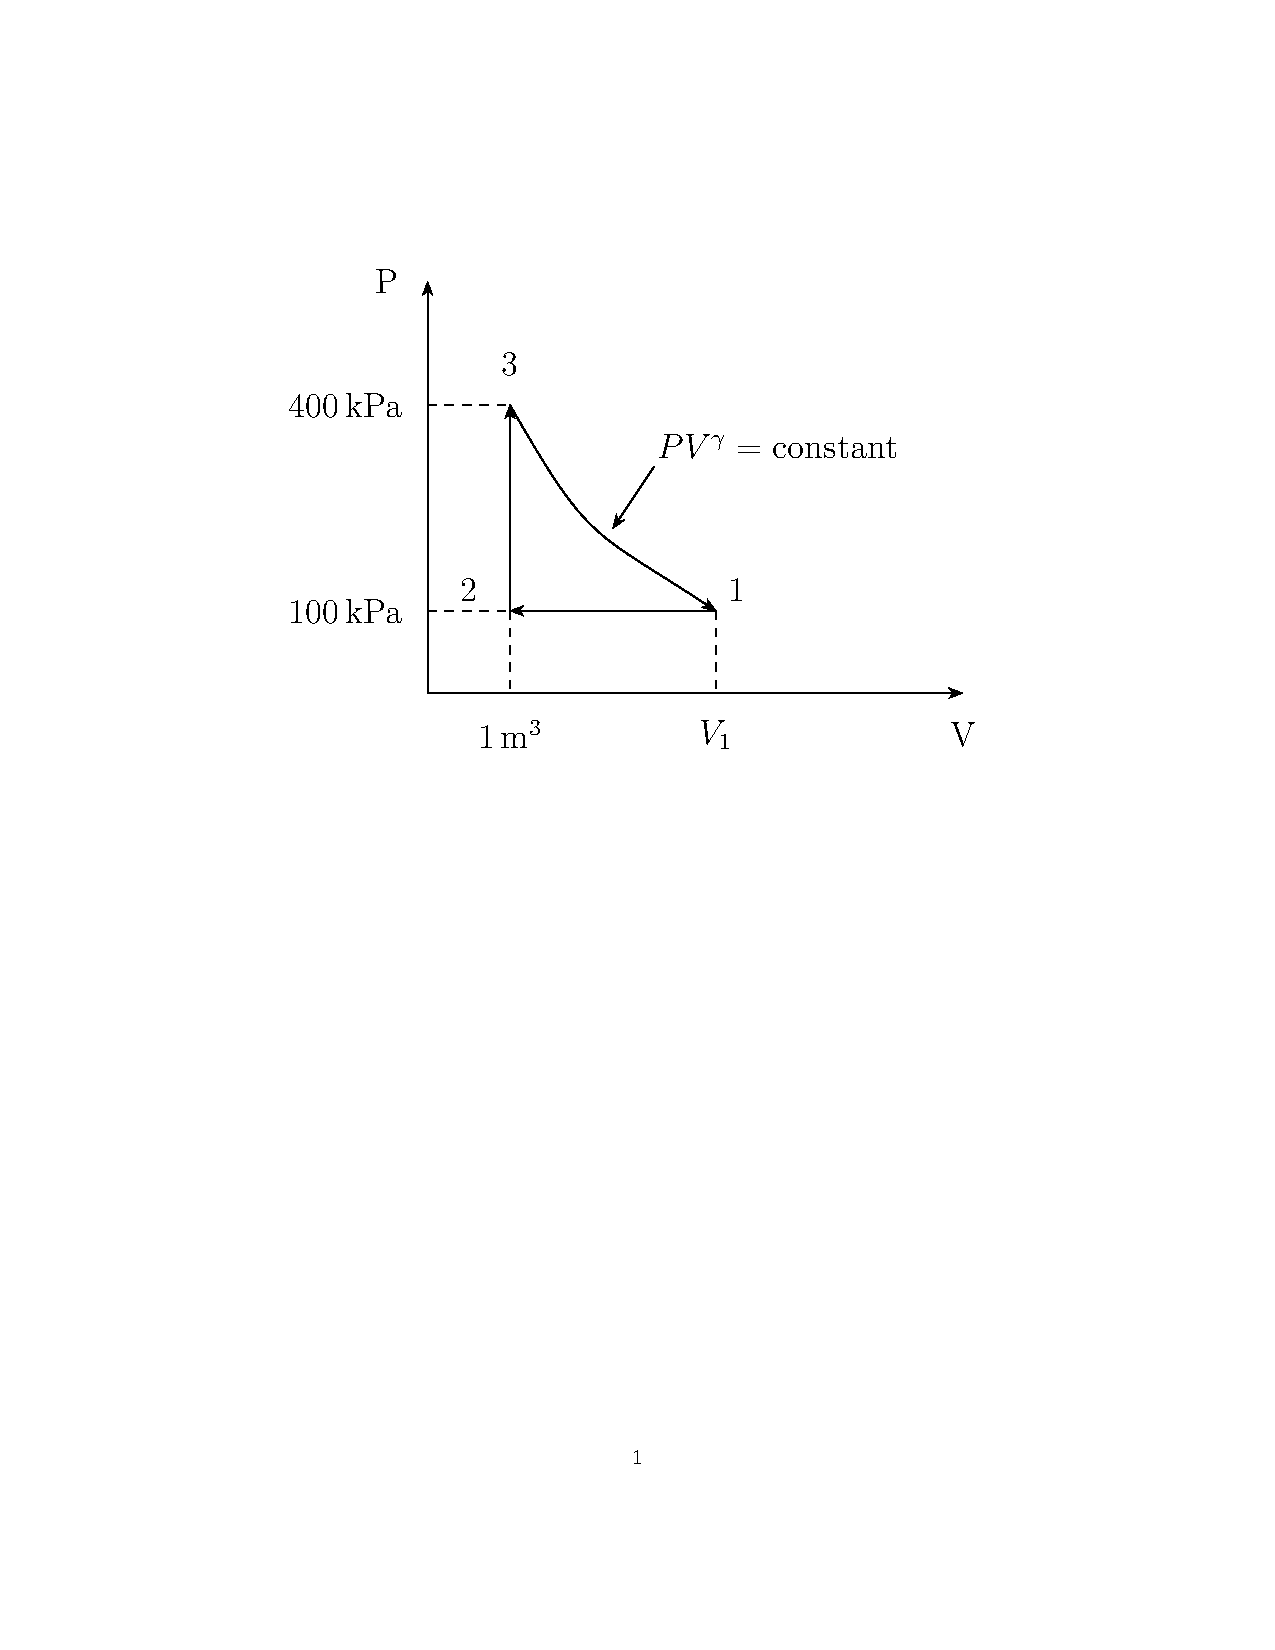
\includegraphics[width=0.7\linewidth]{fig/fig74q/main.pdf}
				\end{minipage}
\end{figure}
		\vspace{-190pt}
	\item The above cycle is represented on $T-S$ plane by\\
		\begin{enumerate}
			\item 
					\begin{figure}[H]
						\begin{minipage}{0.5\textwidth}

	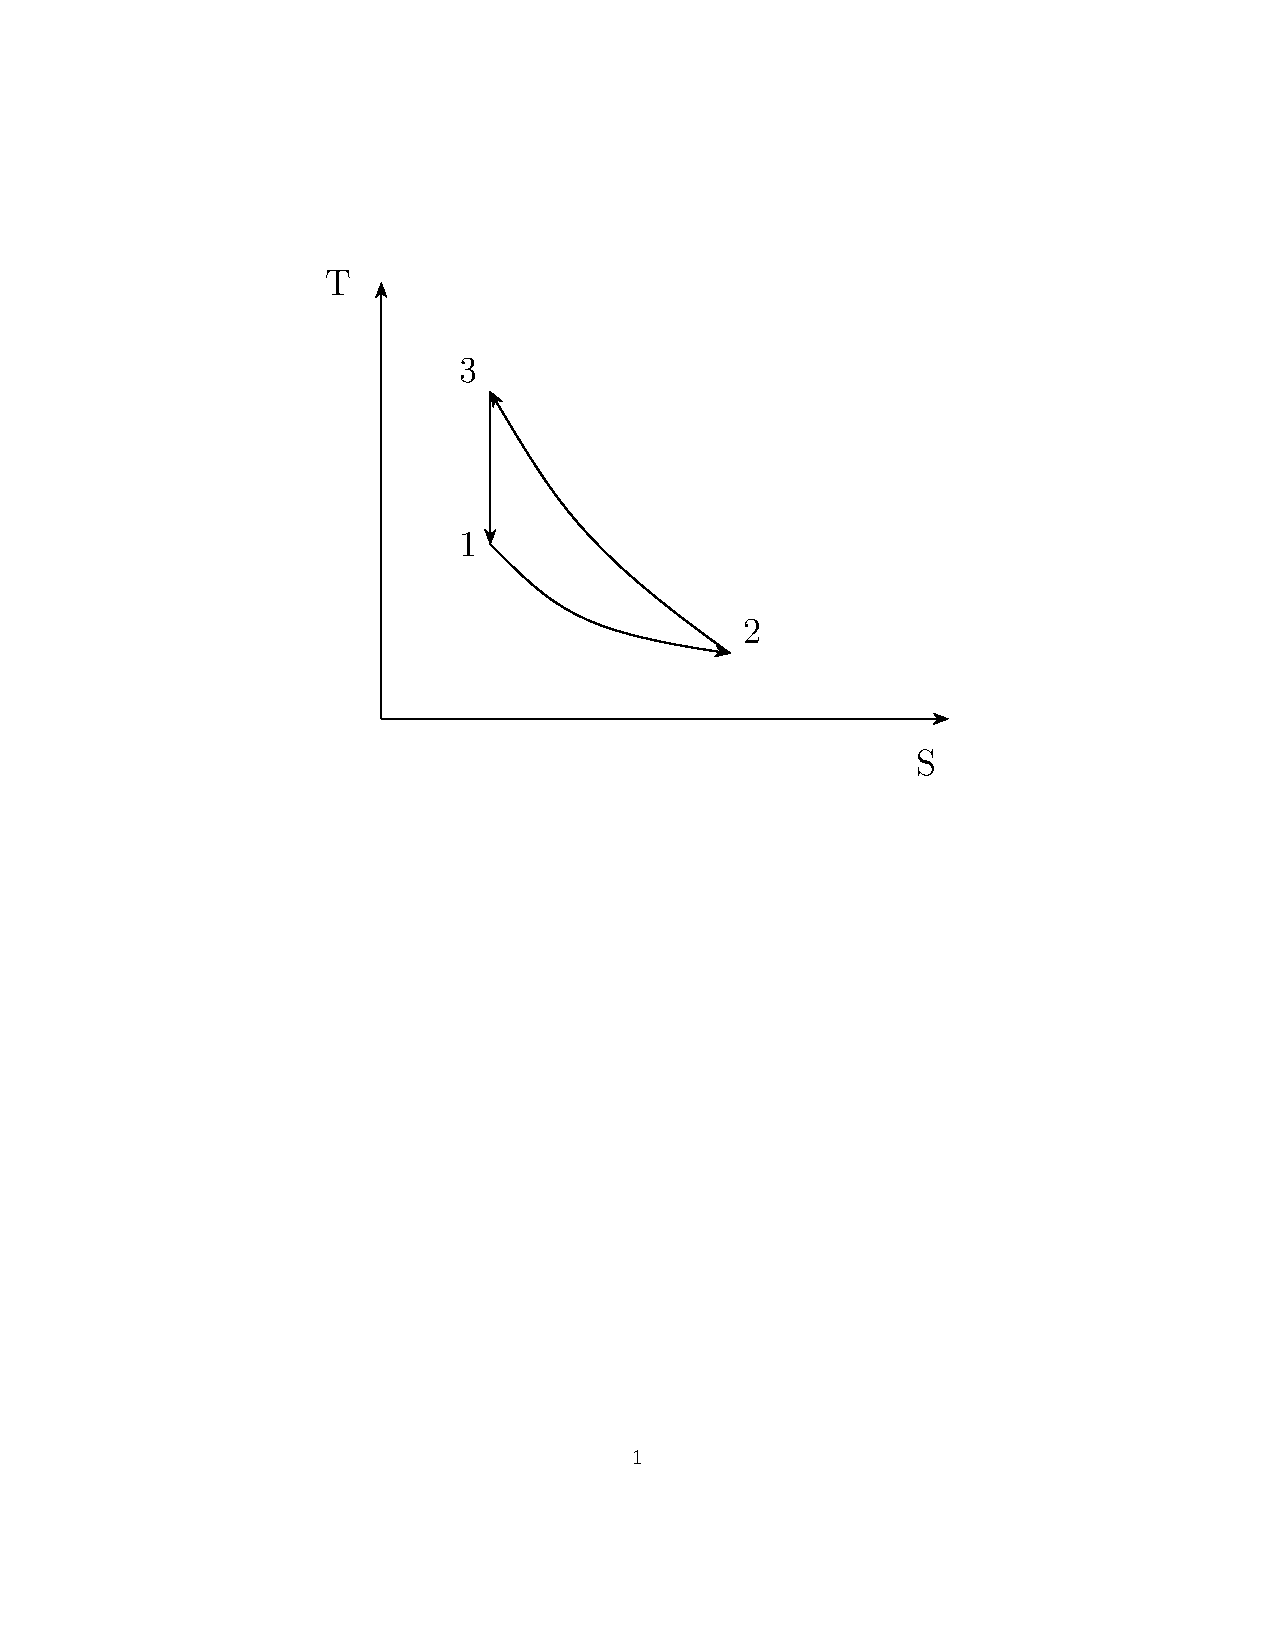
\includegraphics[width=0.7\linewidth]{fig/fig74a/main.pdf}
				\end{minipage}
						\vspace{-180pt}
					\end{figure}
			\item
					\begin{figure}[H]
						\begin{minipage}{0.5\textwidth}
	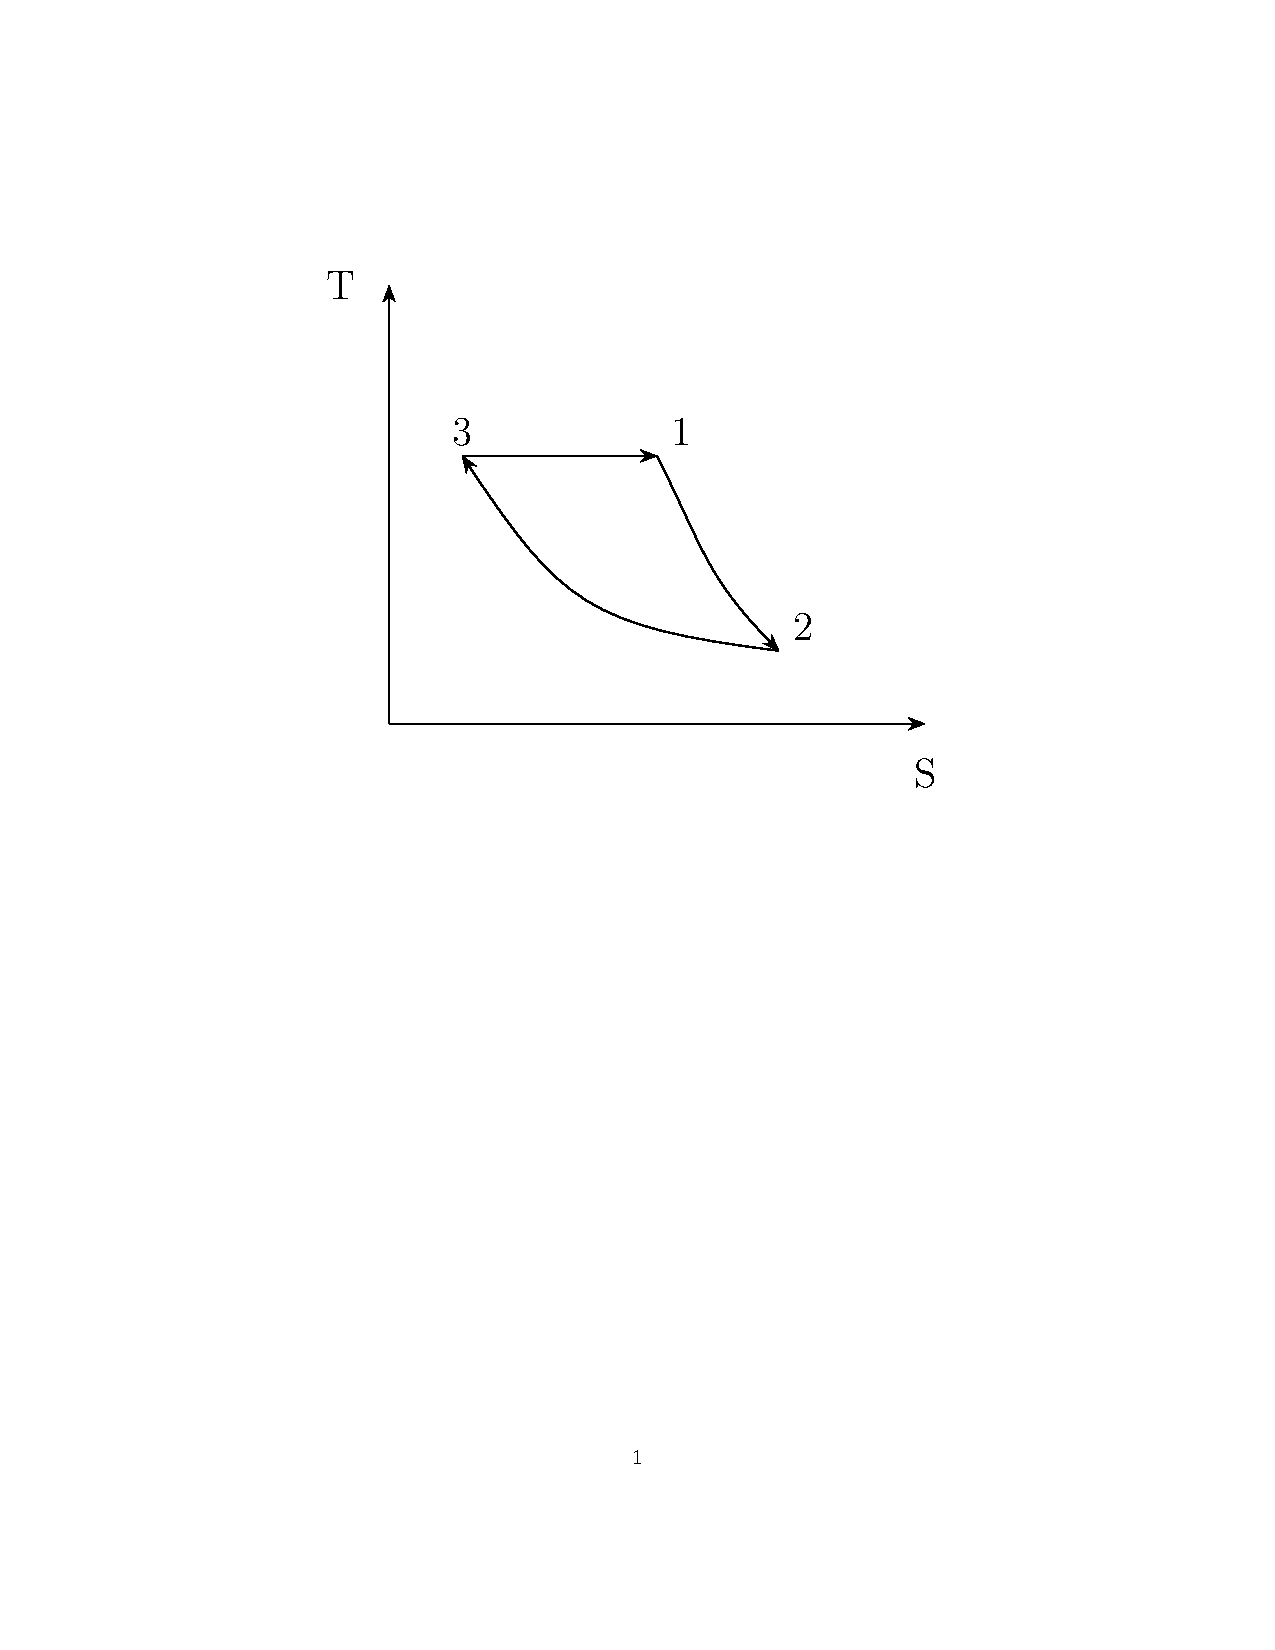
\includegraphics[width=0.7\linewidth]{fig/fig74b/main.pdf}
						\end{minipage}
						\vspace{-180pt}
\end{figure}

			\item
					\begin{figure}[H]
						\begin{minipage}{0.5\textwidth}
	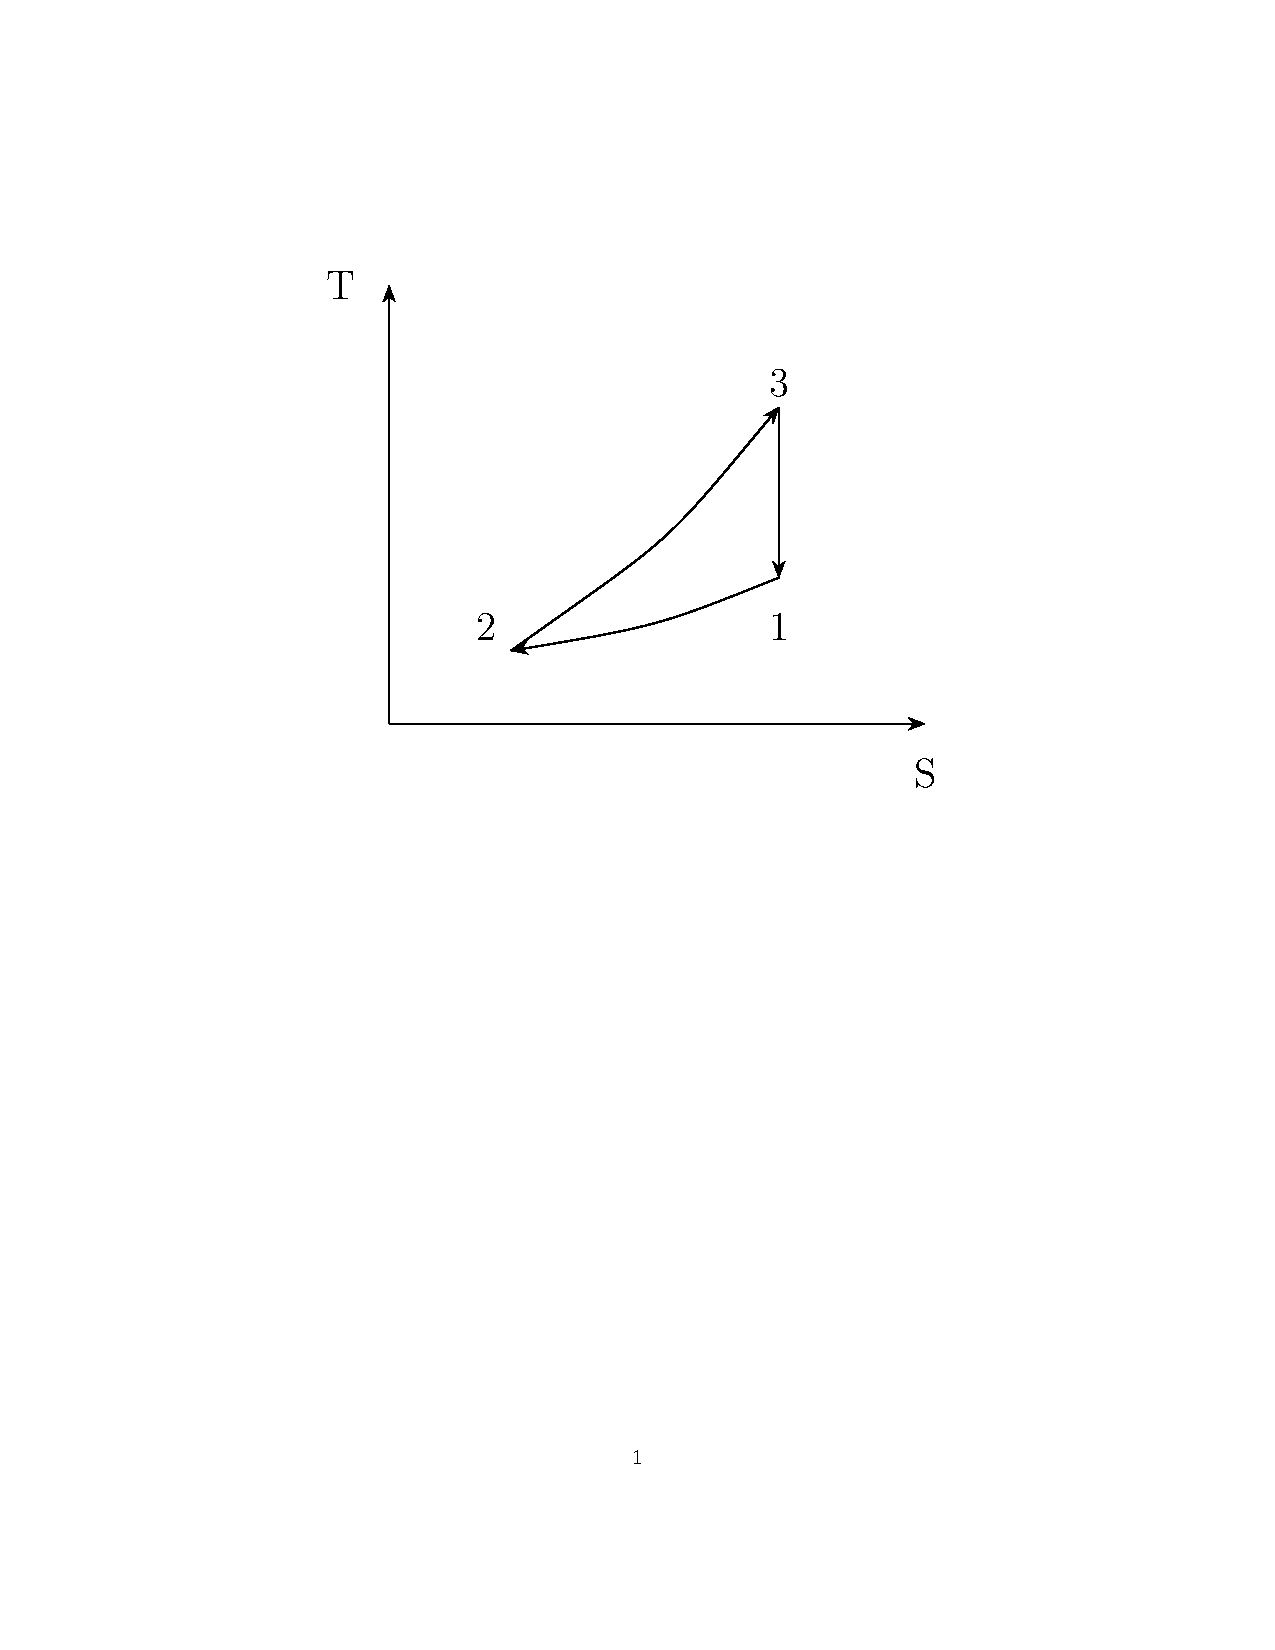
\includegraphics[width=0.7\linewidth]{fig/fig74c/main.pdf}
						\end{minipage}
						\vspace{-180pt}
\end{figure}

			\item
					\begin{figure}[H]
						\begin{minipage}{0.5\textwidth}
	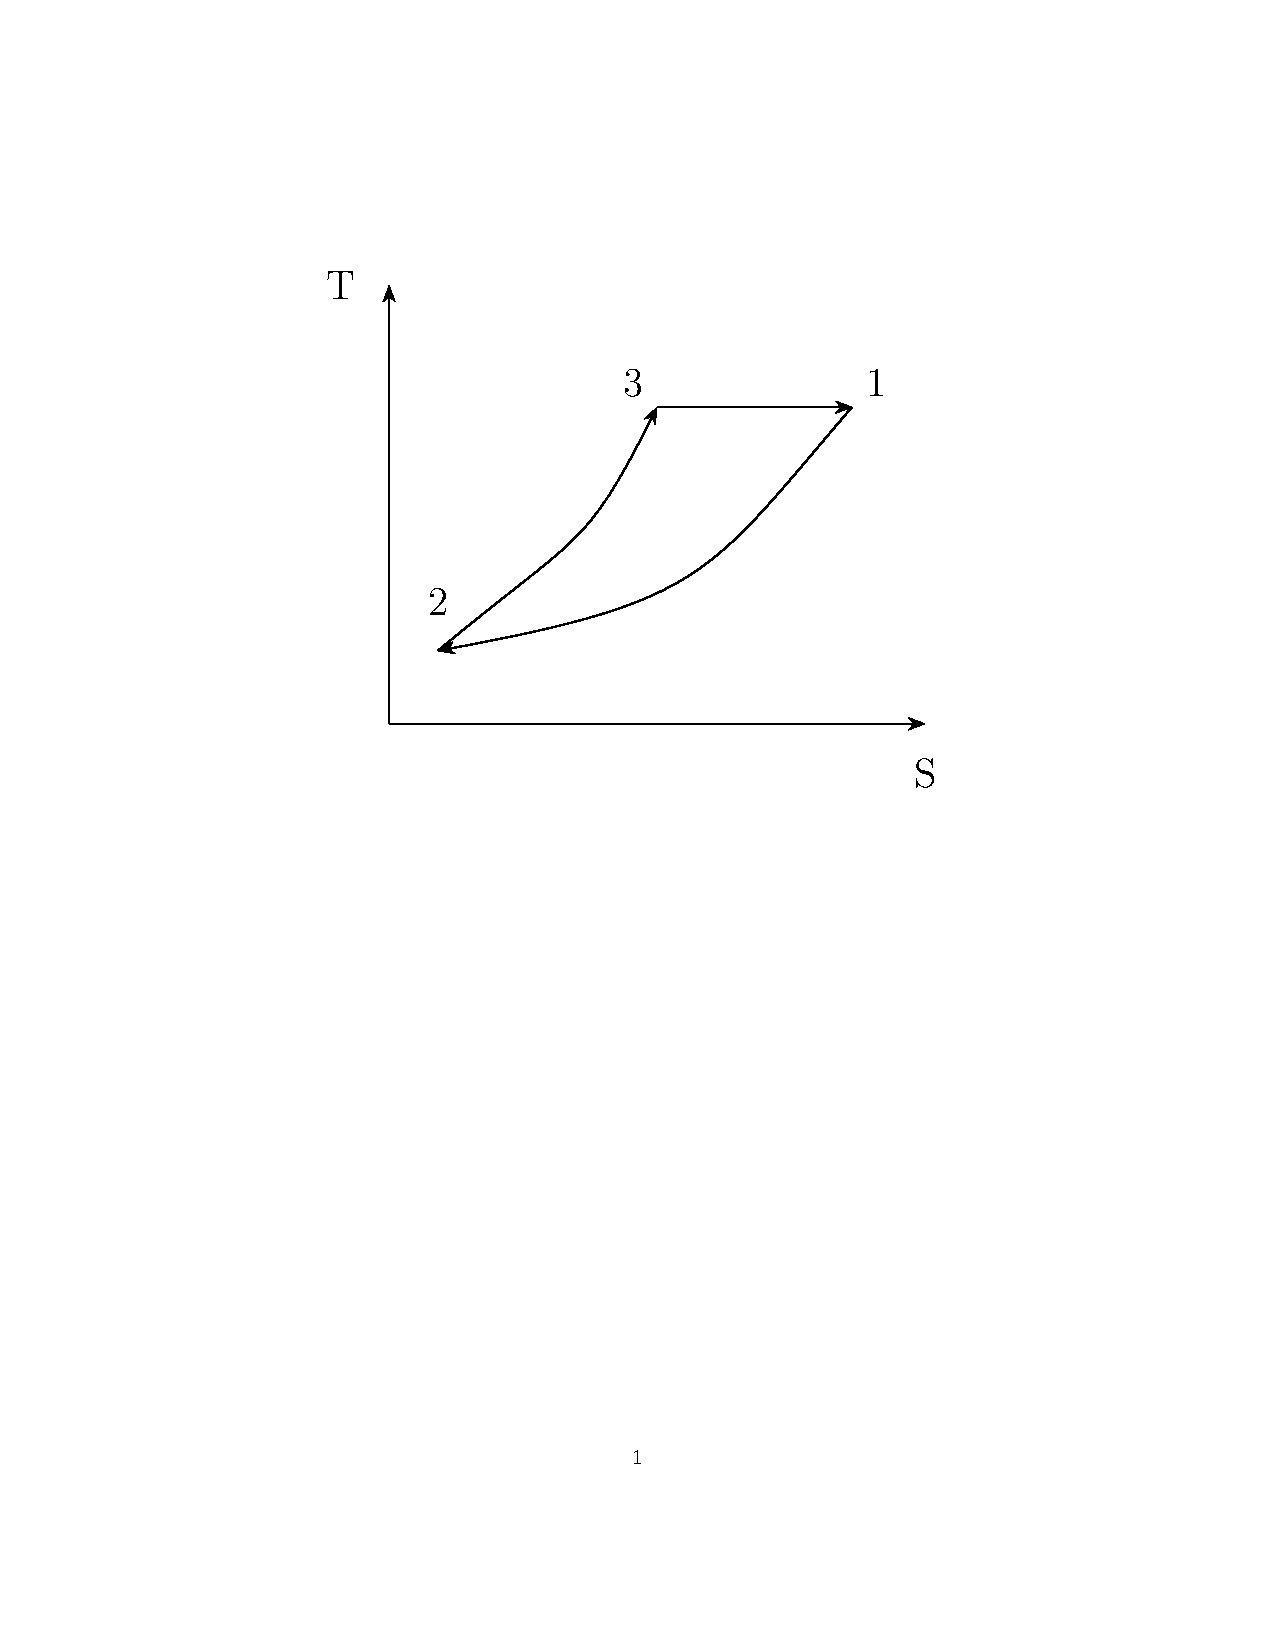
\includegraphics[width=0.7\linewidth]{fig/fig74d/main.pdf}
						\end{minipage}
						\vspace{-190pt}
\end{figure}

		\end{enumerate}
	\item If the soecific heats of the working fluid are constant and the value of specific heat ratio $\gamma$ is $1.4$, the thermal efficiency $\brak{\%}$ of the cycle is 
		\begin{enumerate}
			\item $21$
			\item $40.9$
			\item $42.6$
			\item $59.7$
		\end{enumerate}
		\section*{Linked Answer Questions: Q.76 to Q.85 carry two marks each.}
		Statement for Linked Answer Questions 76 \& 77: \\
		Cosnider a steady incompressible flow through a channel as shown below. \\
			\begin{figure}[H]
	\centering
	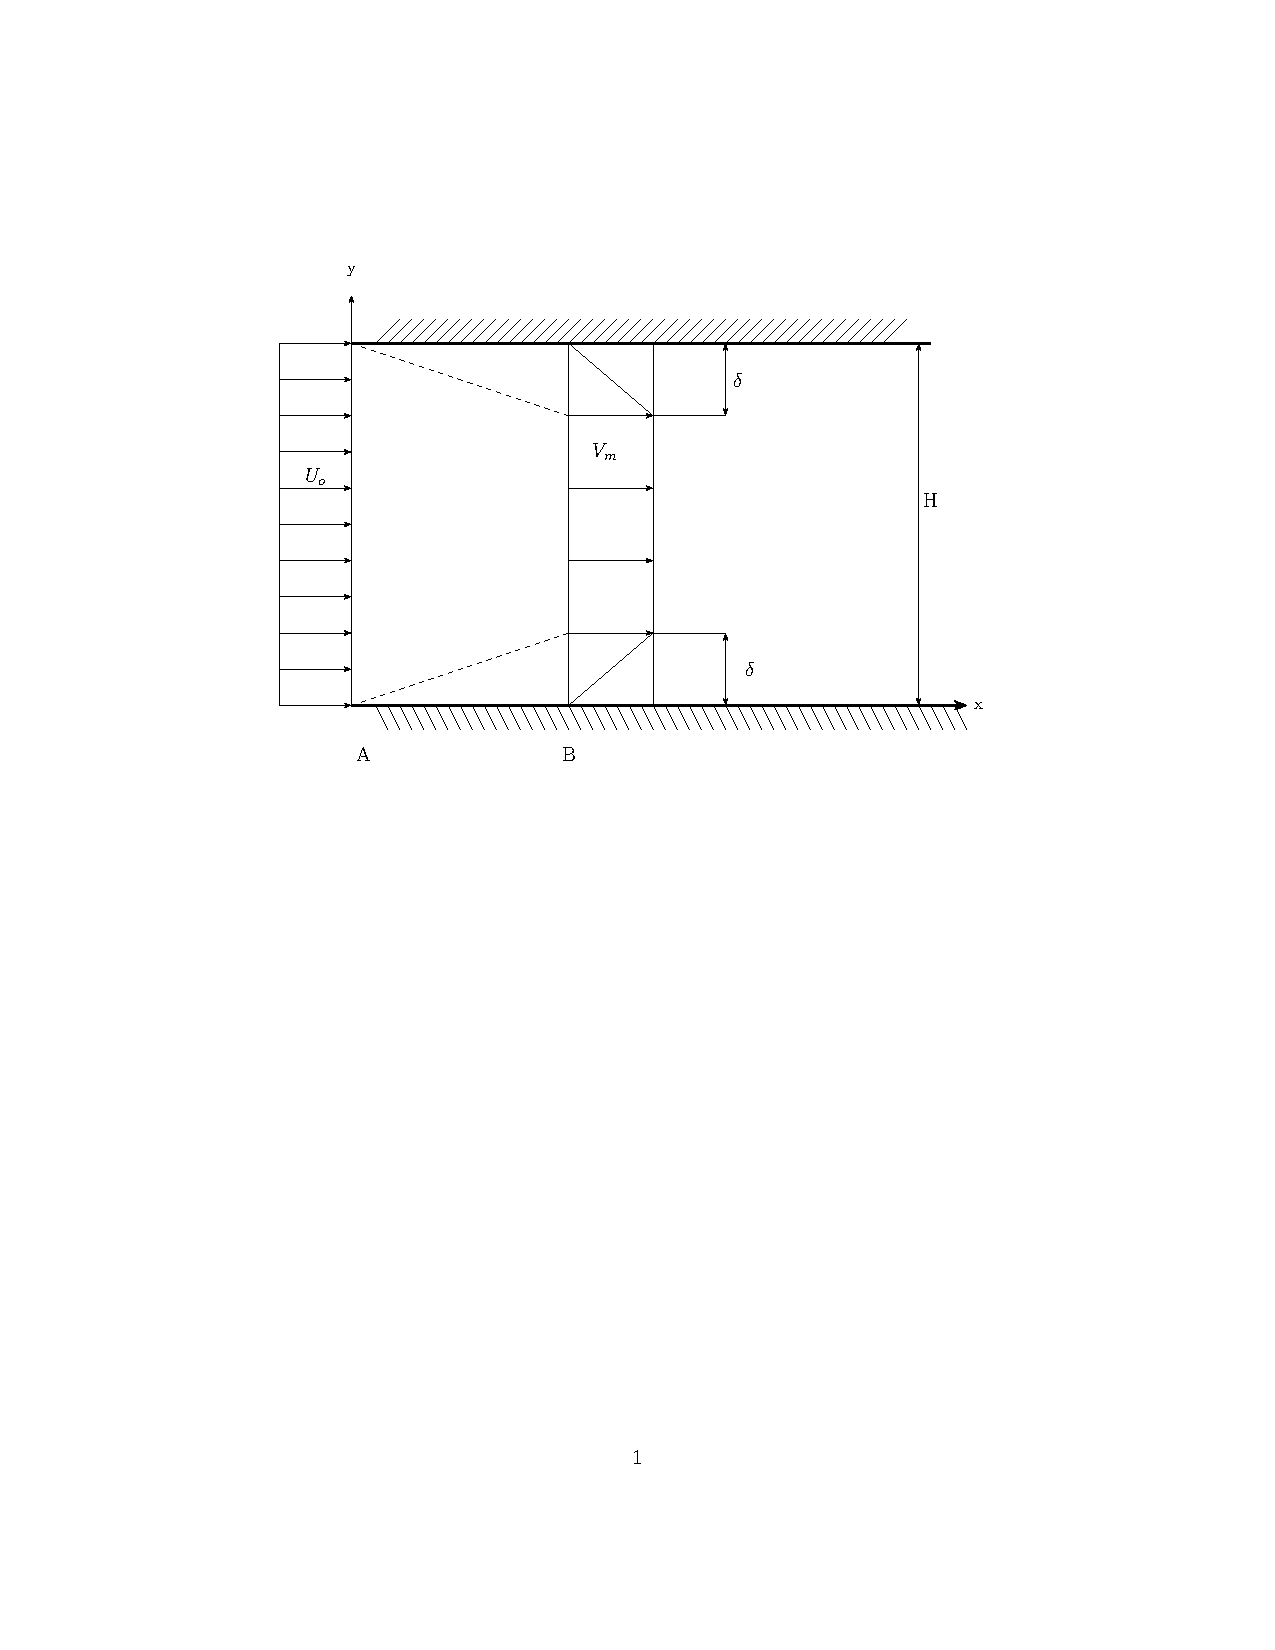
\includegraphics[width=0.7\linewidth]{fig/fig76/main.pdf}
\end{figure}
\vspace{-180pt}

		The velocity proflie is uniform with a value $u_o$ at the inlet section A. The velocity profile at section B downstream is \\
			$u = 
			\begin{cases}
				V_m\frac{y}{\delta}, & 0\le y\le \delta \\
				V_m, & \delta \le y \le H-\delta \\
				V_m\frac{H-y}{\delta}, & H-\delta \le y \le H \\
			\end{cases}$
	
	\item The ratio $V_m/u_o$ is
		\begin{enumerate}
			\item $\frac{1}{1-2\brak{\delta/H}}$
			\item $1$
			\item $\frac{1}{1-\brak{\delta/H}}$
			\item $\frac{1}{\brak{\delta/H}}$ 
		\end{enumerate}
	\item The ratio $\frac{p_A-p_B}{\frac{1}{2}\rho u_{o}^2}$ $\brak{\text{where }p_A \text{and }p_B \text{are the pressures at section A and B, respectively, and }\rho \text{is the denstiy of the fluid}}$ is
		\begin{enumerate}
			\item $\frac{1}{\brak{1-\brak{\delta/H}}^2}-1$
			\item $\frac{1}{\sbrak{1-\brak{\delta/H}}^2}$
			\item $\frac{1}{\brak{1-\brak{2\delta/H}}^2}-1$
			\item $\frac{1}{1+\brak{\delta/H}}$
		\end{enumerate}
		Statement for Linked Answer Questions 78 \& 79: \\
		Consider steady one-dimensional heat flow in a plane of 20 mm thickness with a uniform heat generation of 80 $MW/m^3$. The left and right faces are kept at constant temparature of $160\degree C$ and $120\degree C$ respectively. The plate has a contant thermal conductivity of 200 $W/mK$.
	\item The location of maximum temperature within the plate from its left face is 
		\begin{enumerate}
			\item 15 mm
			\item 10 mm
			\item 5 mm
			\item 0 mm
		\end{enumerate}
	\item The maximum temperature within the plate in $\degree C$ is 
		\begin{enumerate}
			\item 160
			\item 165
			\item 200
			\item 250
		\end{enumerate}
		Statement for Linked Answer Questions 80 \& 81:\\
		\vspace{-70pt}
		\begin{figure}[H]
	\centering
	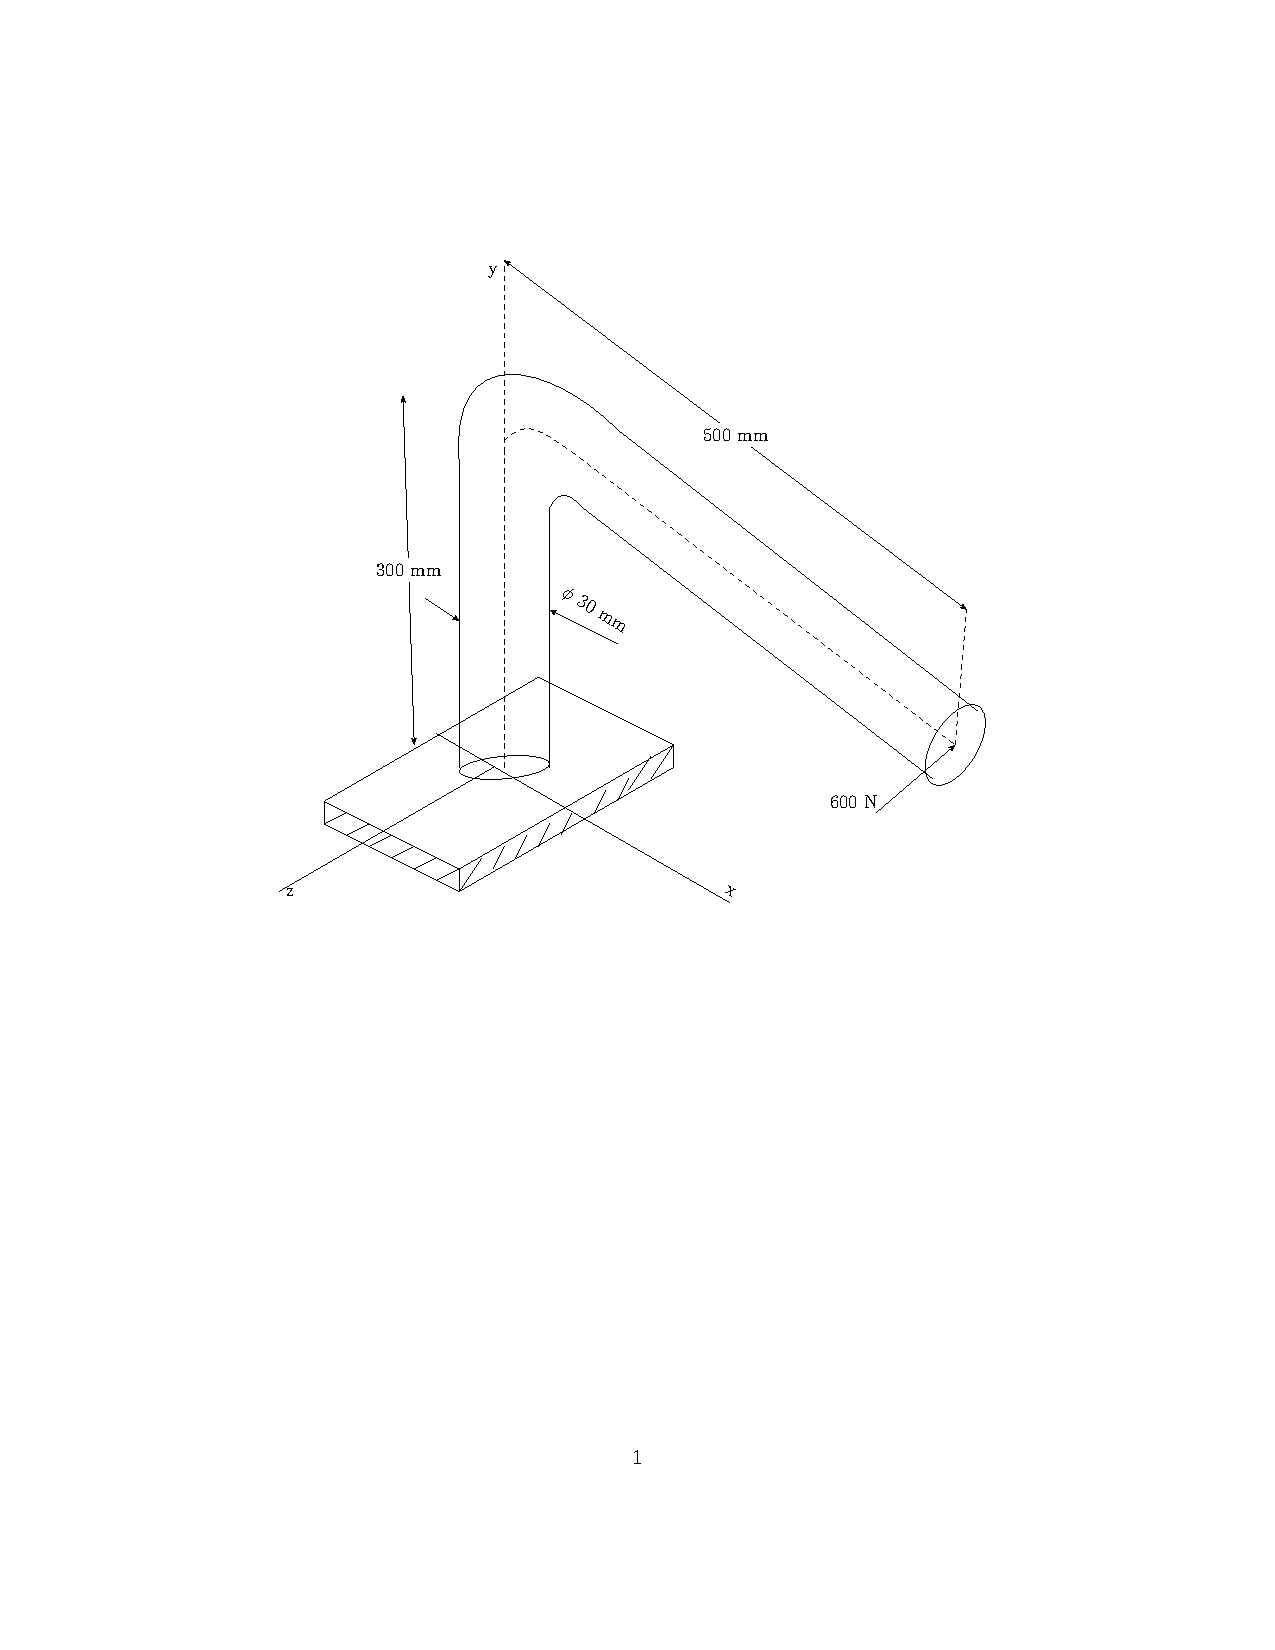
\includegraphics[width=0.7\linewidth]{fig/fig80/main.pdf}
\end{figure}
\vspace{-150pt}

		A machine frame shown in the figure below is subjected to a horizontal force of $600 N$ parallel to z-direction.
	\item The normal and shear stresses in $MPa$ at point $P$ are respectively 
		\begin{enumerate}
			\item $67.9$ and $56.6$
			\item $56.6$ and $67.9$
			\item $67.9$ and $0.0$
			\item $0.0$ and $56.6$	
		\end{enumerate}
	\item The maximum principal stress in $MPa$ and the orientation of the corresponding principal in degrees are respectively 
		\begin{enumerate}
			\item $-32.0$ and $-29.52$
			\item $100.0$ and $60.48$
			\item $-32.0$ and $60.48$
			\item $100.0$ and $-29.52$
		\end{enumerate}
		Statement for Linked Answer Questions 82 \& 83: \\
		A quick return mechanism is shown below. The crank $OS$ is driven ar 2 $rev/s$ in counter-clockwise direction
			\begin{figure}[H]
	\centering
	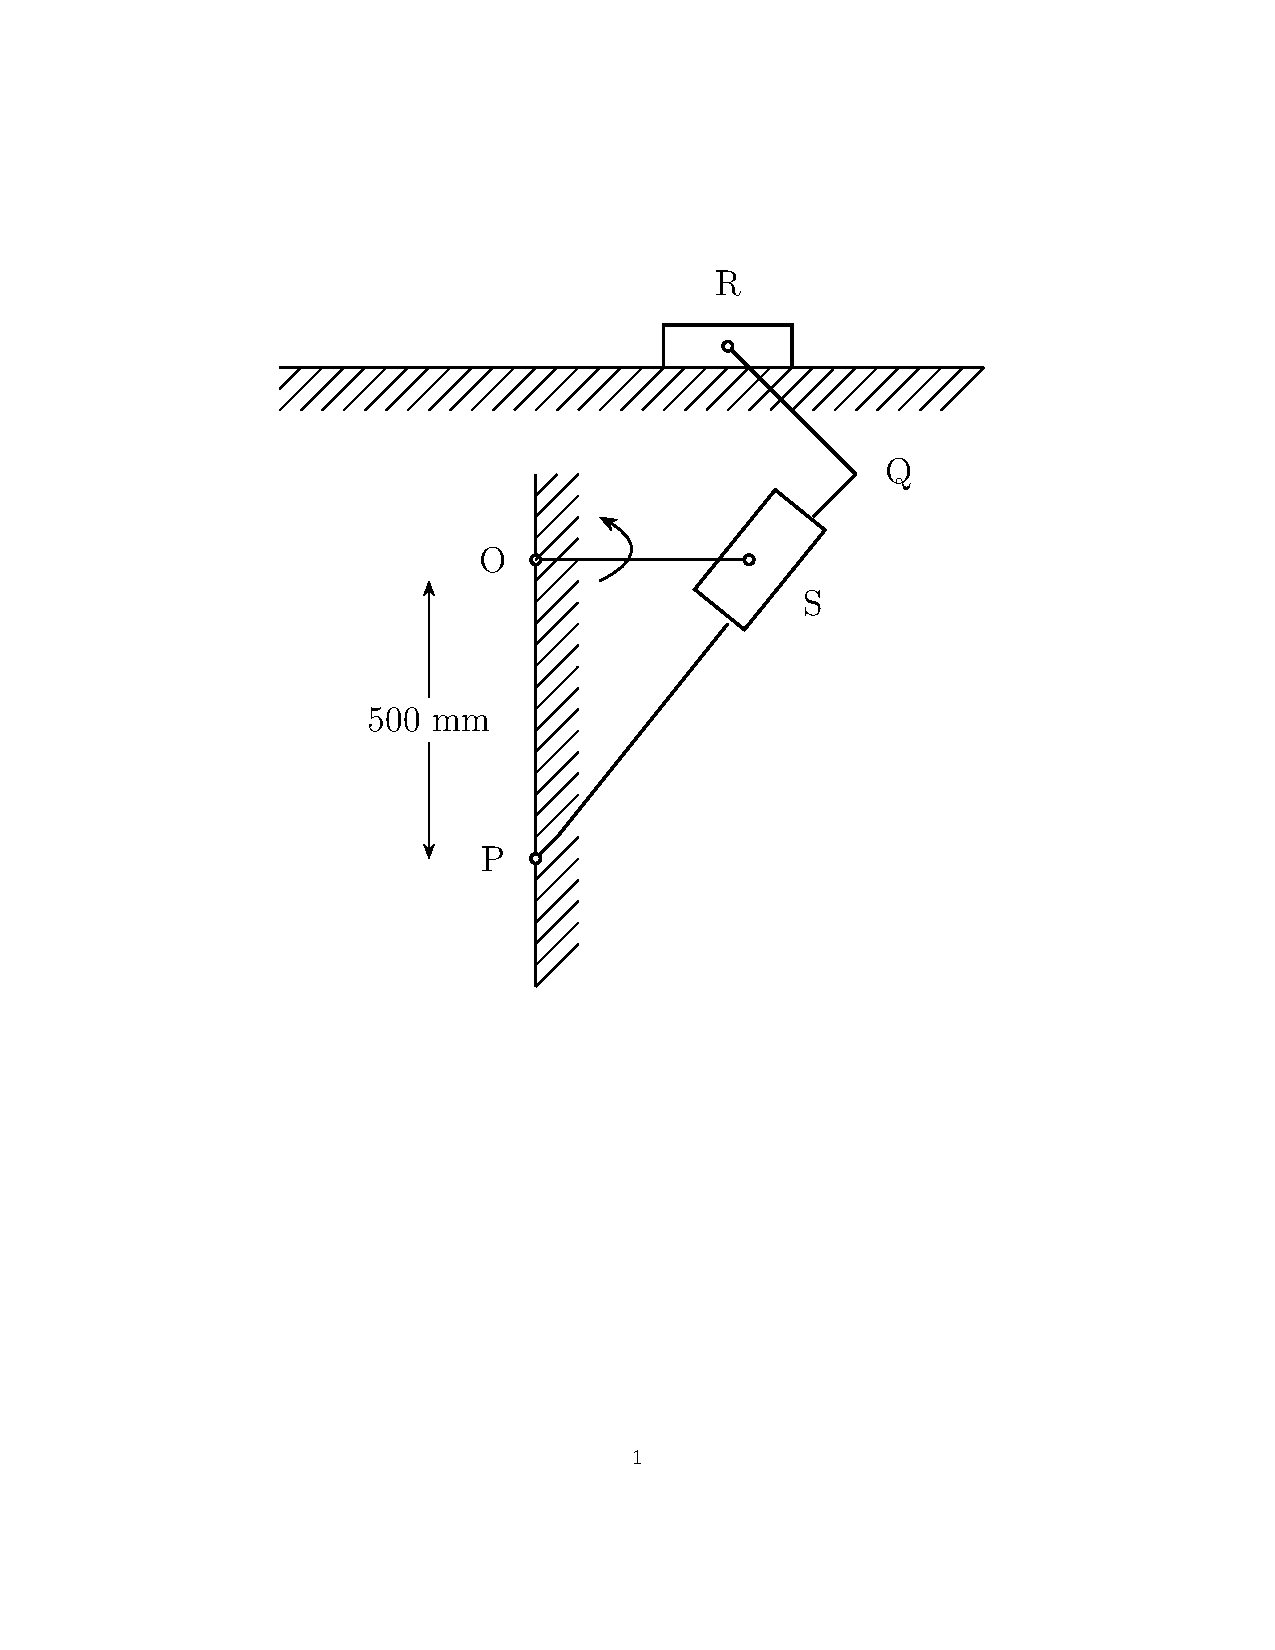
\includegraphics[width=0.7\linewidth]{fig/fig82/main.pdf}
\end{figure}
\vspace{-70pt}

	\item If the quick return ratio is 1:2, then the length of the crank in mm is 
		\begin{enumerate}
			\item 250
			\item $250\sqrt{3}$
			\item 500
			\item $500\sqrt{3}$
		\end{enumerate}
	\item The anugular speed of $PQ$ in $rev/s$ when the block $R$ attains maximum spped during forward stroke $\brak{\text{stroke with slower speed}}$ is 
		\begin{enumerate}
			\item $1/3$
			\item $2/3$
			\item 2
			\item $3$
		\end{enumerate}
		Statement for Linked Answer Questions 84 \& 85: \\
		A low carbon steel bar of 147 mm diameter with a length of 630 mm is being turned with uncoated carbide insert. The observed tool lives are 24 min and 12 min for cutting velocities of 90 m/min and 120 m/min respectively. The feed and depth of cut are 0.2 mm/rev and 2 mm respectively. Use the unmachined diameter to caluculate the cutting velocity. 
	\item When tool life is 20 min, the cutting velocity in m/min is
		\begin{enumerate}
		\item 87
		\item 97
		\item 107
		\item 114
		\end{enumerate}
	\item Neglect over-travel or approach of the tool. When tool life is 20 min, the machining time in min for a single pass is 
		\begin{enumerate}
			\item 5
			\item 10
			\item 15
			\item 20
		\end{enumerate}

\end{enumerate}
\end{document}


